\subsubsection{Key Exchange}
\label{sec:sphinx:keyderivation}

Once path selection as seen in section \ref{sec:path-selection}

Before sending, path selection

% Offline DH key exchange

The sender $A$ picks a random $x\in \mathbb{Z}^*_q$ that is used to derive new keys for every packet.

$A$ randomly picks a path consisting of intermediate nodes $B$, $C$, $D$, and the packet's final destination, $Z$.

$A$ performs an offline Diffie-Hellman (DH) key exchange with each of these nodes and derives shared keys with each of them.

$A$ computes a sequence of tuples $(\alpha_i,s_i,b_i) \in \{ B, C, D, Z \}$ with $\alpha_A = g^x$ and $b_A = h_b(\alpha_A, y_B^{x})$ as follows:

\begin{align}
    \nonumber M_0 & =(\alpha_B,s_B,b_B) = (g^{x b_A},y_B^{x b_A},h_b(\alpha_B,s_B))                                   \\
    \nonumber M_1 & =(\alpha_C,s_C,b_C) = (g^{x b_A b_B},y_C^{x b_A b_B},h_b(\alpha_C,s_C))                           \\
    \nonumber M_2 & =(\alpha_D,s_D,b_D) = (g^{x b_A b_B b_C},y_D^{x b_A b_B b_C},h_b(\alpha_D,s_D))                   \\
    \nonumber M_3 & =(\alpha_Z,s_Z,b_Z)           = (g^{x b_A b_B b_C b_D},y_Z^{x b_A b_B b_C b_D},h_b(\alpha_Z,s_Z))
\end{align}
where $y_B, y_C, y_D$, and $y_Z$ are the public keys of the nodes $B, C, D$, and $Z$, respectively, which we assume to be available to $A$.

\begin{figure}[H]
    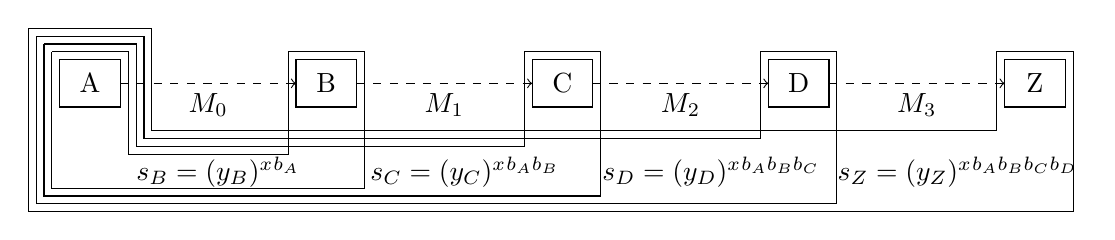
\begin{tikzpicture}
        \def\offset{3}
        \def\nodeWidth{0.77}
        \def\padding{0.93}
        \def\lowerpadding{0.7}
        \def\nodeHeight{0.6}
        \foreach \i\name\bi\packetName in{0/A/0/$M_0$,1/B/$^{b_A}$/$M_0$,2/C/$^{b_Ab_B}$/$M_1$,3/D/$^{b_Ab_Bb_C}$/$M_2$,4/Z/$^{b_Ab_Bb_Cb_D}$/$M_3$} {
                \draw (\i*\offset,0) rectangle (\i*\offset+\nodeWidth,\nodeHeight) node [midway] {\name};

                \ifnum\i>0
                    \draw (-0.1*\i,\nodeHeight+0.1*\i) -- (-0.1*\i,-\padding-0.1*\i) -- (\i*\offset+0.1+\nodeWidth,-\padding-0.1*\i) -- (\i*\offset+0.1+\nodeWidth,\nodeHeight+0.1) -- (\i*\offset-0.1,\nodeHeight+0.1) -- (\i*\offset-0.1,-\lowerpadding+0.1*\i) -- (\nodeWidth+0.1*\i,-\lowerpadding+0.1*\i) -- (\nodeWidth+0.1*\i,\nodeHeight+0.1*\i) -- (-0.1*\i,\nodeHeight+0.1*\i);
                \fi

                \ifnum\i>0
                    \draw [->,dashed] (\i*\offset-\offset+\nodeWidth,0.3) -- (\i*\offset,0.3) node [midway,below] {\packetName} node [midway,below=23pt,shift={(0.13*\i,0)}] {{\smaller$s_{\name}=(y_{\name})^x$\bi}};
                \fi
            }
    \end{tikzpicture}
    \caption{Node $A$ derives shared keys $s_B,s_C,s_D,s_Z$ with node $B,C,D,Z$ using their public keys $y_B,y_C,y_D,y_Z$.}
    \label{fig:sphinx:keyderivation}
\end{figure}
